% poprawione błędy OCR

% kolor zielony jest przeznaczony dla gotyku

% kolor niebieski jest przeznaczony dla łaciny

% słowa dzielone, przenoszone do następnej linijki, są złączone

% w dziesiątej linijce w słowie "raczej" 'e z kreską' zostało zastąpione 'e'

\documentclass[12pt]{article}
\usepackage{fontspec}
\usepackage{amsfonts}
\usepackage{amsmath}
\usepackage{yfonts}
\usepackage{polyglossia}
\usepackage{color}
\usepackage{hyperref}
\usepackage{ifthen}
\usepackage{pdfcomment}
\usepackage[a4paper, left=1cm, right=1cm, top=2cm, bottom=2cm, headsep=1.2cm]{geometry} \defaultfontfeatures{Ligatures=TeX}

\title{G\\ Słownik Lindego\\ t. II s. 17}
\author{Weronika Krakowiak (red.)}

\date{\today}

%%%%%%%%%%%%%%%%%%%%%%%%%%%%%%%%%%%%%%%%%%%%%%%%%%%%%%%

%\setmainfont{Linux Libertine 0}
\setmainfont{Linux Libertine O}

%\setmonofont{DejaVu Sans Mono}
\setmonofont{DejaVu Sans Mono}

% no math
\catcode\&=12

% double oblique hyphen
\newcommand{\doh}[1]{⸗}

%%%%%%%%%%%%%%%%%%%%%%%%%%%%%%%%%%%%%%%%%%%%%%%%%%%%%%%

\usepackage{fontspec}
\usepackage{color}
\usepackage{ulem}
\usepackage{pdfcomment}
\usepackage{hyperref}
\usepackage{graphicx}

%%%%%%%%%%%%%%%%%%%%%%%%%%%%%%%%%%%%%%%%%%%%%%%%%%%%%%%

\begin{document}

\maketitle

\url {http://teksty.klf.uw.edu.pl/26/3/LindeIIGP+2i.djvu?djvuopts=&page=169&zoom=width&showposition=0.2,0.28&highlight=2200,5000,131,193}\\

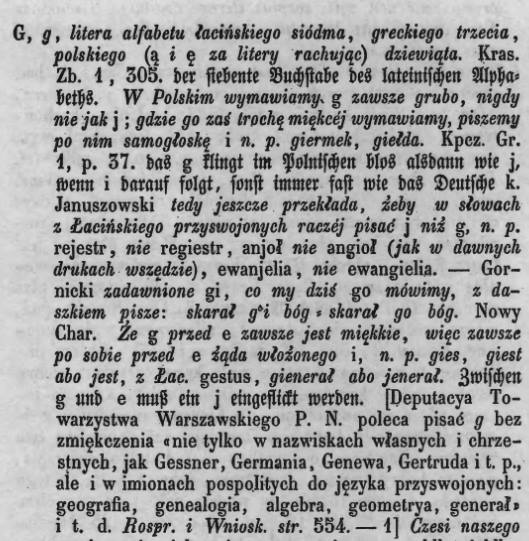
\includegraphics[scale=0.8]{g.jpg}

\newpage
\large
\textup{G,g,} \textit{litera alfabetu łacińskiego siódma, greckiego trzecia}\\ 
\vspace{0.3cm}
\textit{polskiego} \textup{( ą i ę}  \textit{ litery rachuiąc} \textup{) dziewiąta.} \textup{Kras.} \\
\vspace{0.3cm}
\textup{Zb. 1 , 505.} \textcolor{green}{ der siebente Buchstabe des Iateinischen Alphabeths.} \\
\vspace{0.3cm}
\textit{W Polskim wymawiamy,} \textup{g} \textit{zawsze grubo, nigdy} \\
\vspace{0.3cm}
\textit{nie jak} \textup{j ;} \textit{gdzie go zaś trochę miękcej wymawiamy, piszemy} \\
\vspace{0.3cm}
\textit{po nim samogłoskę } \textup{i} \textit{ n. p. giermek, giełda.} \textup{Kpcz. Gr.} \\
\vspace{0.3cm}
\textup{4, p. 57.} \textcolor{green}{ das} \textit{g} \textcolor{green}{ klingt im Polntschen blos alsdann wie} \textup{ j,} \\
\vspace{0.3cm}
\textcolor{green}{wenn} \textup{ i } \textcolor{green}{darauf folgt, sonst immer. fast wie das Deutsche}  \textit{k.} \\
\vspace{0.3cm}
\textup{Januszowski} \textit{tedy jeszcze. przeklada, żeby, w słowach} \\
\vspace{0.3cm}
\textit{z Łacińskiego przyswojonych raczej pisać} \textup{j} \textit{niż} \textup{g,} \textit{n. p. }\\
\vspace{0.3cm}
\textup{rejestr,} \textit{ nie} \textup{ regie'str, anjoł } \textit{ nie} \textup{ angioł } \textit{(jak w dawnych} \\
\vspace{0.3cm}
\textit{drukach- wszędzie),} \textup{ ewanjelia , } \textit{nie} \textup{ ewangielia. - Gornicki} \\
\vspace{0.3cm}
\textit{zadawnione} \textup{ gi, } \textit{ co my dziś } \textup{go} \textit{ mówimy, z daszkiem} \\
\vspace{0.3cm}
\textit{pisze: skarał g*i bóg} \doh{} \textit{skarał go bóg.} \textup{Nowy} \\
\vspace{0.3cm}
\textup{Char.} \textit{Że} \textup{g} \textit{przed} \textup{e} \textit{zawsze jest miękkie, więc zawsze} \\
\vspace{0.3cm}
\textit{po sobie przed} \textup{e} \textit{żąda włożonego} \textup{i,} \textit{n. p. gies, giest} \\
\vspace{0.3cm}
\textit{abo jest, z Łac.} \textcolor{blue}{gestus,} \textit{gienerał abo jenerał.} \textcolor{green}{Zwischen}\\
\vspace{0.3cm}
\textup{g} \textcolor{green}{und} \textup{e} \textcolor{green}{muß ein} \textup{j} \textcolor{green}{eingefiickt werden.} \textup{ [Deputacya Towarzystwa} \\
\vspace{0.3cm}
\textup{Warszawskiego P. N. poleca pisać} \textit{g} \textup{bez} \\
\vspace{0.3cm}
\textup{zmiękczenia «nietylko w nazwiskach własnych i chrzestnych,} \\
\vspace{0.3cm}
\textup{jak Gessner, Germania, Genewa, Gertruda i t. p.,} \\
\vspace{0.3cm}
\textup{ale i w imionach pospolitych do języka przyswojonych:} \\
\vspace{0.3cm}
\textup{geografia, genealogia, algebra, geometrya, generał»} \\
\vspace{0.3cm}
\textup{i t. d.} \textit{Bospr. i Wniosk. str. 554.- 4} \\


\end{document}

%%% Local Variables: 
%%% coding: utf-8-unix
%%% mode: latex
%%% TeX-master: t
%%% TeX-PDF-mode: t
%%% TeX-engine: xetex
%%% End: 
